\section{ЦЕЛЬ И ЗАДАЧИ РАБОТЫ} %поменять с программами местами

\textit{Целью} работы является создание комплекса программ для решения ОДУ и СДУ и её дальнейшая отладка на модельных задачах.
Безусловно, в этот программный комплекс должны входить различные явные и неявные методы решения ОДУ, графический
пользовательский интерфейс, парсер математических выражений и многое другое.

В связи с этим можно сформулировать следующие задачи, представленные на рисунке \ref{fig:goals}:
\begin{enumerate}
    \item Выполнить обзор существующих программ для решения ОДУ, выявить их основные недостатки;
    \item Реализовать стандартный набор явных, неявных, вложенных, диагональных, а так же многошаговых методов решения ОДУ;
    \item Разработать парсер математических выражений, который можно использовать для ввода задачи Коши. Адаптировать парсер для
    применения его в задачах химической кинетики, в частности для ввода химических компонент, химических реакций, скоростей
    химических реакций и другой информации, необходимой для моделирования химической кинетики;
    \item Разработка графического пользовательского интерфейса, дизайна программы и инструментов для генерации pdf-отчётов о решениях
    задач;
    \item Выбрать оптимальные по времени и точности схемы для моделирования различных химических процессов на основе разработки ПО
    для решения систем ОДУ явными и неявными методами;
    \item Сравнение с существующими программами для решения ОДУ и СДУ.
\end{enumerate}

\begin{figure}
    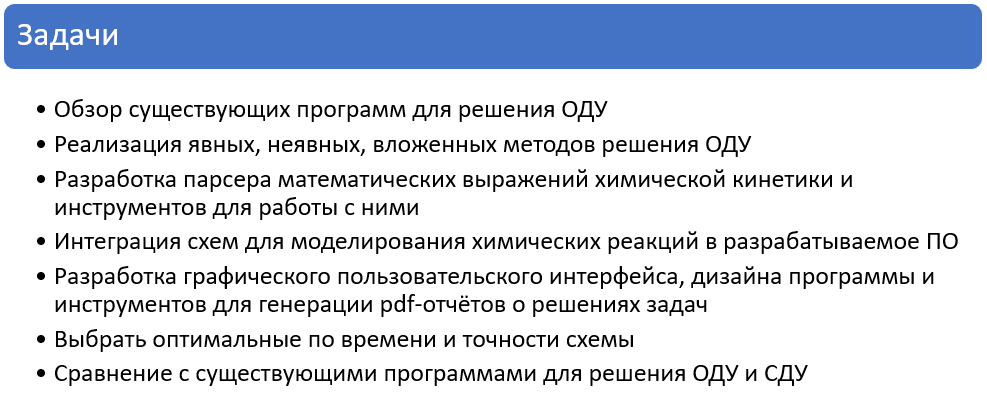
\includegraphics[width=15cm]{2-02-goals}
    \caption{Основные задачи проекта}
    \label{fig:goals}
\end{figure}

После выполнения данных задач, можно приступить к разработке отдельных модулей для работы с задачами физики, биологии и т.д. Так же
планируется работа над кроссплатформенностью.

Идея работы, основные элементы алгоритмов и результаты тестовых испытаний были изложены 11 апреля 2023 г. на 49-й конференции
Гагаринских чтений
по направлению №7 ("Математические методы в аэрокосмической науке и технике")
секции №3 ("Теоретическая механика и дифференциальные уравнения"). Темой доклада было "Моделирование и оптимизация химической кинетики
на базе схем Рунге-Кутты для решения жёстких систем ОДУ". Тезисы доклада будут опубликованы в сборнике трудов.

Так же была подана заявка на участие в 23-й международной конференции по вычислительной механике и современным прикладным
программным системам (ВМСППС'2023), которая будет проводиться с 4 по 13 сентября 2023 г. 